\documentclass[runningheads]{llncs}
\usepackage[utf8]{inputenc}

\usepackage{graphicx}
\usepackage{amsmath}
\usepackage{amssymb}
\usepackage{arydshln}
\usepackage{xcolor,ulem}
% Used for displaying a sample figure. If possible, figure files should
% be included in EPS format.
%
% If you use the hyperref package, please uncomment the following line
% to display URLs in blue roman font according to Springer's eBook style:
% \renewcommand\UrlFont{\color{blue}\rmfamily}

\setlength{\parskip}{0cm}
\setlength{\parindent}{1em}

\newcommand{\reals}{\mathbb{R}}

\newcommand{\comment}[3]{{\color{#1} {\bf #2 :} #3}}
%\newcommand{\comment}[3]{}  % suppress comments
\newcommand{\kui}[1]{\comment{blue}{Kui}{#1}}
\newcommand{\yoav}[1]{\comment{red}{Yoav}{#1}}

\renewcommand\floatpagefraction{.99}
\renewcommand\topfraction{.99}
\renewcommand\bottomfraction{.99}
\renewcommand\textfraction{.1}   
\setcounter{totalnumber}{50}
\setcounter{topnumber}{50}
\setcounter{bottomnumber}{50}
\setlength{\abovecaptionskip}{0pt}
\setlength{\belowcaptionskip}{0pt}

\title{Towards explainable automated Neuroanatomy}
\author{Kui Qian, Beth Friedman, David Kleinfeld, Yoav Freund}
\date{January 2022}

\begin{document}

\maketitle

\begin{abstract}
  A fundamental goal of neuroanatomy is the identification of brain
  structures.  Manual identification of structures is based on the
  spatial distribution of cell shape, size, orientation and density.
  With new technology it is possible to image entire brains at high
  resolution.  However, manual identification of structures in these
  massive datasets is prohibitively time consuming.  We present a
  machine learning method for automatic detection of brain structures. Our approach is based on diffusion maps, in combination with hand-picked features, and Adaboost for combining the features. Our method is robust against brain to brain variation and details of neuronal staining.
  Our method produces structure detections together with their explanation. This  that the human anatomist and the computer interact to improve the detection of structures and the addition of new structures.
  
  %We translate each cell image into a feature vector that
  %includes aspect ratio, orientation and area, as well as additional
  %features derived using a graph Laplacian. The algorithm uses the
  %statistical distribution of these features vectors to identify brain
  %structures.
\end{abstract}

\section{Main}

\begin{enumerate}
\item {\bf Summary:} We propose a system for detecting anatomical structures in the mouse brain. Our system takes as input high-resolution images of aligned sections. It produces as output the estimated center of mass (COM) for each structure. Each detection is assigned a confidence. High confidence structures are associated with a visual explanation.
\item {\bf Significance for Neuroanatomy}
Does not have to be very detailed. Target audience is ML.
\begin{itemize}
\item Importance and History
\item Manual detection of brain structures has two major drawbacks, the first is the amount of time needed by an anatomist. The second is inconsistencies between anatomists. Automatic detection has the potential of reducing the time and improving the consistency for this task.
\item Challenges: Variability of images
    \begin{itemize}
        \item biology: animal to animal, gender, generally alien across species, transgenic (differentions to genome due to gene expression)
        \item technical: staining, sectioning (mechanical, optical)
    \end{itemize}
\end{itemize}
\item {\bf Explainable AI} Black box approaches focus on finding an accurate end-to-end mapping. As such, these approaches are hard to interrogate when they fail. In contrast, we take an explainable-detector which allows the anatomist to understand {\em why} the ML made particular decisions. This benefits both sides ...

\item{\bf Cell based approach}  Most CNN-based method of image analysis are based on the concept of a sliding window. This implies that any explanation provided by the CNN is based on the content of one or more windows. Windows need to be large enough to capture the image statistics. This means that a typical window contains 10-100 cells.
On the other hand, anatomist base their analysis on cytoarchitecture, which, in turn, is based on the shapes of individual cells and the relationshp between them. This makes it harder for the anatomist to understand the decisions of the detector.

To remedy this problem and make the detections explainable, we use individual cells as our basic unit. 
\end{enumerate}

\subsection{System design}

The trained system is a collection of structure detectors. Each structure is a known anatomical entity. To train the detectors we combine three sources of information:
\begin{itemize}
    \item {\bf Images of aligned sections:} The Nissl images of XX brains are the primary information source. They are also by far the largest at XXX GB per brain.
    \item {\bf The Atlas} is a representation of the shape of each structure and the relative locations of the structures. The atlas was constructed through a concensus ....
    \item {\bf COMs for individual brains:} For XX brains we had an anatomist locate the COM ....
\end{itemize}

The overall design of the system is shown in Figure xxx
\begin{enumerate}
\item{\bf Dimensionality reduction}
An image of a single cell is typically around 50$\times$50 pixels, or a 2500 dimensional vector. The dimension of this representation is too high for effective machine learning. We therefor seek a dimensionality reduction mapping. This mapping consists of three parts:
\begin{enumerate}
    \item {\bf Normalization:} We normalize the image of the cell in three ways. We 
    shift the grey-levels so that the mean is XXX, scale the grey levels so that the standard deviation is YYY, and rotate the image so that the long axis of the cell is in angle zero. The three parameters associated with the normalizations define three features.
    \item {\bf Standard shape features}: we use the Hu features: x,y,z...
    \item{ \bf  Diffusion maps}: Diffusion Mapping~\cite{Belkin, Coifman} is a non-linear dimensionality reduction method that is based on a graphical representation of the data and on the Laplace operator on graphs. 
\end{enumerate}

which is based on cells as the basic unit. Doing so provides an explanation for the detector's decision. We use unsupervised learning to find a dimensionality reducing mapping for cell shapes. We make efficient use of manual annotations by estimating the shape of each structure from a few brains and anatomists. We leverage this information in the detector training by having the anatomist identify the location of the center of mass for each structure.
\end{enumerate}
\section{Results}
\begin{itemize}
    \item Detection results, with confidence levels, consistency with Beth.
    \item {\bf Explaining detections} The explanation of the detection is expressed in terms of cells whose shape gives evidence to the structure.
\item {\bf Cell shape parametrization} Uses a combination of Hu moments and dimensionality reduction using eigen-maps.
\begin{itemize}
    \item Eigen-maps learn a dimensionality reducing mapping cell shape to a ten dimensional representation.
    As it is an unsupervised method it requires no human labeling. We take advantage of the very large number of cells in single brain.
    \item Each brain creates a different mapping, however, the mappings can be made consistent by adding a linear transformation. This creates a stable parametrization and makes the detections more consistent.
\end{itemize}

\end{itemize}


\section{Methods}
\begin{enumerate}
\item{\bf Characterizing Cytoarchitecture} uses Difference between the CDFs for inside and outside of each structure (based on manually annotated structure boundaries). 
\item {\bf Structure detectors} Combine the difference-of-CDF features using boosted trees (XGBoost). Each structure has a corresponding detector.
\item {\bf Structure detection confidence} The confidence of structure detections is measured by the prediction margin and by the sharpness of the detection peak.
\item{\bf Image based alignment} (rough alignment) is used to find and approximate alignment.
\item {\bf Detection based alignment} Starting with the locations of the landmarks from the image based alignment we perform a rough search for the detection peak, followed by a finer grid for estimating the detection confidence.
\item{\bf Detection and alignment refinement} Using the confident detections we improve the alignment. Improved alignment constraints the locatioan of the structure and allows using less confident detections.
\end{enumerate}

\section{writeup from 2022/01/21}
The disagreements on anatomical classification implies the need to a metric of confidence on the detection and characterization of brain structures.
The difficulty or ease of detecting a structure is variable. 
In any particular brain, some structures are detected consistently by anatomists while others are not.
The challenge in making the system usable to the anatomists is first to automatically detect structures and second, to provide an explanation for its detections and an associated confidence.

Our goal in the design of the system is to create models of the brain
that can be explained to, and modified by, anatomists. In other words,
we take a white box, rather than a black box approach.

This impacts the design in several important ways. First, image
analysis methods in general, and CNNs in particular, are based on
concept of a sliding window. In other words, the basic unit of
analysis is a rectangular area, whose location is indpendent of the
content of the image. In contrast our analysis unit is the image of a
single cell.~\footnote{When cells are overlapping we sometimes get
  the image of several scells as the unit.} By annotating cells we
visually explain to the anatomist the basis for the computer's
decision.

Second, we represent each cell by a set of features. the basic 
features are size, aspect ratio, and orientation. To characterize the
cell shape beyond these basic features, we use an unsupervised
learning method to find a dimensionality reducing mapping from cell
image to ten additional parameters. We demonstrate that this
unsupervised method provides a consistent parameterization across
brains and across imaging modalities.

Third, explaining structure detection (xxxx).



\section{Adaptive parametrization of cell shapes}
\label{sec:DM}
In this section we describe the two main technical contributions of this
paper: a method for learning a cell-shape feature-set that is optimized
for a particular brain, and a method for mapping between feature-sets
from different brains. Both methods are {\em unsupervised}, in other
words, the input to these methods are sets of sections with no
annotation or alignment.

The first step is to segment individual cells from the section
image. For this we use a locally adaptive variant of
Otsu's method~\cite{otsu1979threshold}. This step is not perfect, over and under segmentations are
common. However, our method relies on the statistical properties for
many cells, which greatly reduces the sensitivity of the analysis to
segmentation errors. 
Cell patches are typically $50\times 50$ pixels which is a highly
redundant representation. The second step is to
map the cell image to a less redundant low-dimensional representation. Our goal here
is to find a small set of features (10) that represent shapes of cells
from a given brain. Our learned features provide a better representation 
of cells shapes which contrast with the feature extraction stage in~\cite{chen2019active}, 
which uses a pre-trained CNN (Inception-BN). 


We use Diffusion Maps
(DM)~\cite{belkin2003,coifman2005geometric}~\footnote{{\tt
    https://github.com/DiffusionMapsAcademics/pyDiffMap}} to find a
low dimensional representation of cell shapes. While DM has gained
popularity in many applications, the only work we are aware of
regarding the use of DM for cell shape analysis is in the context of
differentiation lineages~\cite{haghverdi2015diffusion}.
The public implementation of DM is excellent. However, it is limited to datasets that
fit in computer memory. As we typically extract from each brain
hundreds of millions of cells, we need an efficient way to create a
small number of representative patches.  We use a streaming version of
the Kmeans++~\cite{arthur2006k} seeding algorithm followed with a few
iterations of Kmeans. Figure~\ref{fig:kmeans} shows samples of the
original cell images and of cells after normalizing
rotation, Kmeans++ and Kmeans averaging.
\begin{figure}[t]
  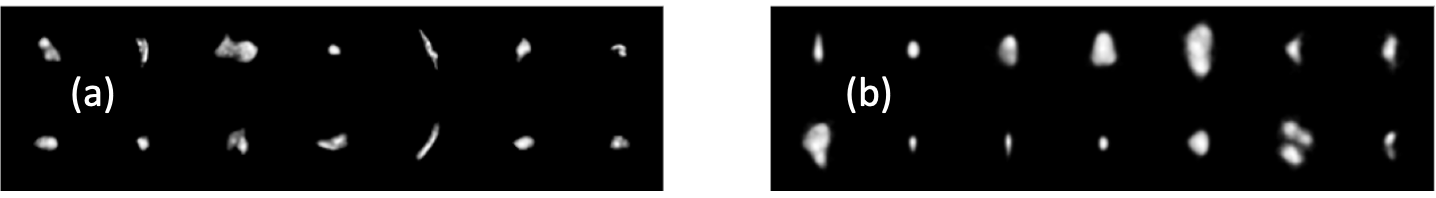
\includegraphics[width=\textwidth]{Images/CellImages.png}
\caption{{\bf (a)} a sample of Cell patches,
  {\bf (b)}  a sample of the orientation-normalized, Kmeans-reduced and averaged cell images.}
\label{fig:kmeans}
\end{figure}

DM~\cite{coifman2005geometric} creates a continuous
non-linear mapping from single cell patches into a ten component
feature vector. The ten components correspond to ten most dominant
(lowest non-zero eigenvalue) eigen-vectors of the Laplace-Beltrami
operator. We conceptualize the DM of a population of cells as
a ten dimensional cloud of patches, each patch placed at the location
defined by the corresponding feature vector. By projecting this cloud
onto a two dimensional plane, we generate a visualization of the patch
cloud (see figure~\ref{fig:diffusionmap}).

After inspecting patch clouds from several brains, it became clear
that the clouds corresponding to different brains are similar. More
precisely, the clouds all have similar shapes when projected on
different planes, but the order of and orientation can be
different. This gave us the idea that there might be a single {\em
  universal} set of features, such that one can map the shape-features from
any brain to this universal set of features.

Such a universal set of features provides several benefits. First, it
provides a way to visualize the difference between regions in terms of
the density, types and orientations of cells. This gives
the anatomist a way to understand the decisions made by the computer
and potentially correct them. This is in contrast with black box
methods such as deep neural networks which provide no explanations of
their decisions.

\begin{figure} [t]
  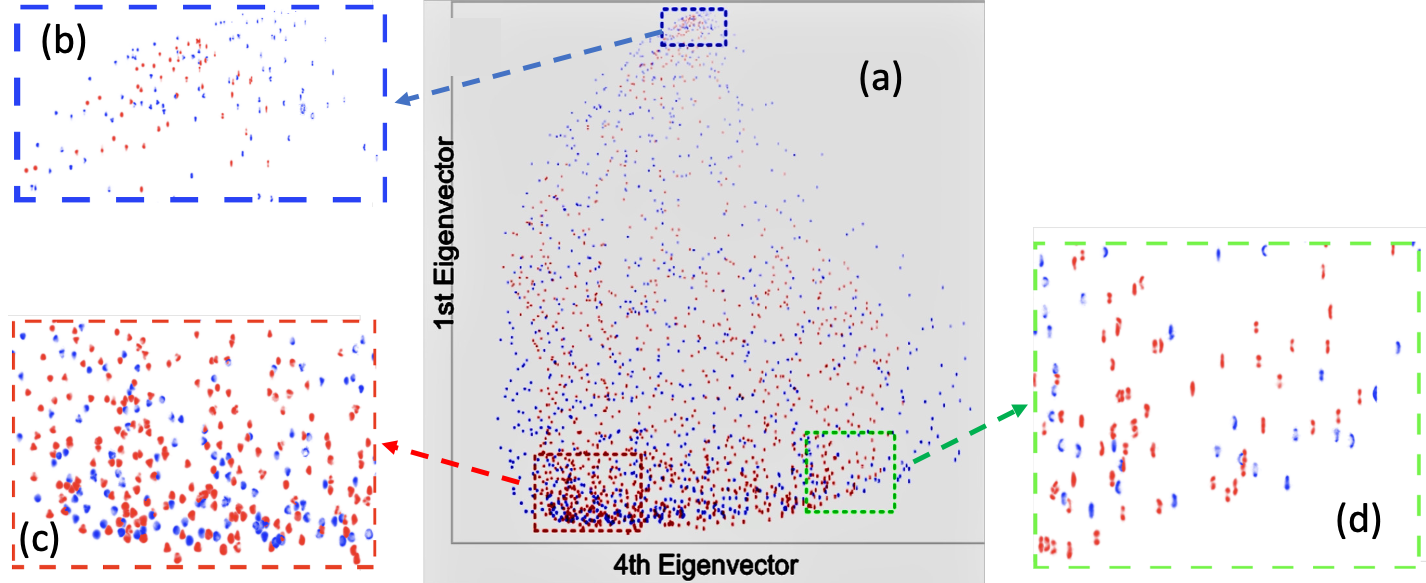
\includegraphics[width=\textwidth]{Images/Scatter.png}
\label{fig:diffusionmap}
\caption{{\bf Projecting the patch cloud and universal features}. This
  figure demonstrates the continuous mapping generated by DM. {\bf
    (a)} shows the projection of two patch clouds on the first and
  fourth eigenvectors produced by DM. The red patches correspond to
  cells stained by Thionin and imaged using brightfield, the blue
  patches correspond to cells stained with Neurotrace blue and imaged
  using fluorescent imaging. The brightfield cloud has been
  transformed to match the fluorescent cloud. Observe that the shape
  of the clouds match closely. Further, the insets show that the cell
  shapes match as well.  {\bf (b)} corresponds to very
  small cells. {\bf (c)} correspond to large and round cells, and {\bf
    (d)} correspond to thin cells or a row  of 2-3 cells.}
\end{figure}
Second, using a universal set of features decouples any downstream processing from
variations in section preparation and imaging. Such decoupling is particularly
valuable when switching between different imaging modalities such as
fluorescence vs. brightfield. In the next section we show that
structure Detection benefits from the universal set of features.

After the transformation to universal features, patch clouds from
different imaging modalities overlap almost perfectly. This is
demonstrated in figure~\ref{fig:diffusionmap}. 
The transformations we used to between patch clouds are simple affine
transformations. To find a good transformation between two clouds we
use a simple RMS-based formulation (details in Appendix A). The
important thing is that this transformation, like DM, is
unsupervised. All that is needed are the two DM feature vectors and
the cell patches. The result is an unsupervised learning method for
learning features. The first step is DM and the second step is finding
a transformation from the generated feature set to a universal feature
set.

\section{Supervised Learning}

\section{Computer generated suggestions of new landmarks}

 \bibliographystyle{splncs04}
 \bibliography{Reference}

\appendix

%\section{Experimental setup}
%Brightfield brain images are from sectioned brains of P56, male
%C57BL/6 mice with a thicknesses of microns and a 0.46-micron
%resolution. The Nissl substance were stained by thionin, which
%highlights neural textures across brains. These stained objects were
%segmented by OpenCV into units called as cells in this paper. We then
%normalized cells by padding them into patches with three sizes of
%large, medium and small.

\section{Transformation between Diffusion Maps}
\subsection{Problem Description and Solution}
The mathematical formulation of finding a linear transformation between two different diffusion maps can be described as follows: Given a set of vector pairs $(a_1,b_1),\ldots,(a_n,b_n)$ where each of the vectors $a_i,b_i$ are in a $d$ dimensional space $R^d$,  find an offset vector $\mu \in r^d$ and a linear transformation $M$ which is a $d \times d$ matrix so that the following cost function is minimized:

\begin{equation}
\label{cost_function}
    cost(\mu, M) = \frac{1}{n}\sum_{i=1}^n||\mu + Ma_i - b_i||_2^2
\end{equation}

We first compute the hessian matrix of ~\ref{cost_function} with respect to $\mu$ and $M$ to see if the problem can be directly solved.
\begin{equation}
\label{hessian_1}
    \frac{\partial^2 cost(\mu, M)}{\partial \mu \partial \mu^T} = 2I \rightarrow p.d
\end{equation}
\begin{equation}
\label{hessian_2}
    \frac{\partial^2 cost(\mu, M)}{\partial M \partial M^T} = \frac{2}{n}\sum_{i=1}^na_ia_i^T \rightarrow p.s.d
\end{equation}

The results show that both hessian matrices are Positive Semi-definite matrices and thus we can find the solution by setting derivatives to 0. We have:
\begin{equation}
    (\frac{1}{n}\sum_{i=1}^na_ia_i^T - \frac{1}{n}\sum_{i=1}^na_i\times \frac{1}{n}\sum_{i=1}^na_i^T)M^T = \frac{1}{n}\sum_{i=1}^na_ib_i^T - \frac{1}{n}\sum_{i=1}^na_i\times \frac{1}{n}\sum_{i=1}^nb_i^T
\end{equation}




%\subsection{Cost Function}
%\begin{equation*}
%\begin{aligned}
%    cost(\mu, M) = \frac{1}{n}\sum_{i=1}^n||\mu + Ma_i - b_i||_2^2 = \frac{1}{n}\sum_{i=1}^n(\mu + Ma_i - b_i)^T(\mu + Ma_i - b_i) \\
%    = \mu^T\mu + 2\mu^TM\frac{1}{n}\sum_{i=1}^na_i - 2\mu^T\frac{1}{n}\sum_{i=1}^nb_i + \frac{1}{n}\sum_{i=1}^na_i^TM^TMa_i - \frac{2}{n}\sum_{i=1}^na_i^TM^Tb_i + \frac{1}{n}\sum_{i=1}^nb_i^Tb_i
%\end{aligned}
%\end{equation*}
%
%\subsection{Derivative}
%\begin{equation*}
%    \frac{\partial cost(\mu, M)}{\partial \mu} = 2\mu^T + \frac{2}{n}\sum_{i=1}^na_i^TM^T - \frac{2}{n}\sum_{i=1}^nb_i^T
%\end{equation*}
%\begin{equation*}
%    \frac{\partial cost(\mu, M)}{\partial M} = \frac{2}{n}\sum_{i=1}^na_i\mu^T + \frac{2}{n}\sum_{i=1}^na_ia_i^TM^T - \frac{2}{n}\sum_{i=1}^na_ib_i^T
%\end{equation*}
%
%\subsection{Hessian}
%\begin{equation*}
%    \frac{\partial^2 cost(\mu, M)}{\partial \mu \partial \mu^T} = 2I \rightarrow p.d
%\end{equation*}
%\begin{equation*}
%    \frac{\partial^2 cost(\mu, M)}{\partial M \partial M^T} = \frac{2}{n}\sum_{i=1}^na_ia_i^T \rightarrow p.s.d
%\end{equation*}
%
%\subsection{Results}
%Let $\frac{\partial cost(\mu, M)}{\partial \mu} = 0$, we have:
%\begin{equation*}
%    2\mu^T + \frac{2}{n}\sum_{i=1}^na_i^TM^T - \frac{2}{n}\sum_{i=1}^nb_i^T = 0
%\end{equation*}
%\begin{equation}
%    \mu^T = \frac{1}{n}\sum_{i=1}^nb_i^T-\frac{1}{n}\sum_{i=1}^na_i^TM^T
%\end{equation}
%
%Let $\frac{\partial cost(\mu, M)}{\partial M} = 0$, we have:
%\begin{equation*}
%    \frac{2}{n}\sum_{i=1}^na_i\mu^T + \frac{2}{n}\sum_{i=1}^na_ia_i^TM^T - \frac{2}{n}\sum_{i=1}^na_ib_i^T = 0
%\end{equation*}
%\begin{equation}
%    \frac{1}{n}\sum_{i=1}^na_i\mu^T = \frac{1}{n}\sum_{i=1}^na_ib_i^T - \frac{1}{n}\sum_{i=1}^na_ia_i^TM^T
%\end{equation}
%
%Put (6) into (7), we have:
%\begin{equation*}
%    (\frac{1}{n}\sum_{i=1}^na_ia_i^T - \frac{1}{n}\sum_{i=1}^na_i\times \frac{1}{n}\sum_{i=1}^na_i^T)M^T = \frac{1}{n}\sum_{i=1}^na_ib_i^T - \frac{1}{n}\sum_{i=1}^na_i\times \frac{1}{n}\sum_{i=1}^nb_i^T
%\end{equation*}

\section{Pseudo-code for Finding Significant Regions}
\begin{enumerate}
  \item Calculate the statistical significance map of the whole 3D shape relative to the background as $Mask$. Traverse the whole shape with a cube (200 microns cubed) by a step size of 100 microns.
  \item Define $M$ to mark regions in the 2D shape and $R$ to record cubes of each region.
  \item Find seeds and expand them to foreground regions according the following rules:
  		\begin{itemize}
			 \item Find the cube with the highest KS significance in $Mask$ of unmarked regions ($M==0$) as the seed. Append that cube to a list of potential starting cubes $C$.
			 \item Pop one starting cube from $C$. Starting from the chosen cube, slide by a stride of half window size to get 8-connected neighborhood cubes as foreground candidates.
 			 \item The foreground candidates are added to the foreground and the list $C$ if $dist(x,S_B )>\alpha \cdot dist(x,S_F)$ where $S_F$ represents the CDFs of cells in the foreground and $S_B$ represents the CDFs of cells in the background. $\alpha$ is set to be 3.
			 \item Repeat the above two steps until the list $C$ is empty.
		\end{itemize}
  \item Find 100 regions via 200 micron cubed seeds, then find 30 regions via 100 micron cubed seeds.
  \item After finding regions, for pairs of regions in $R$:
 		 \begin{itemize}
			 \item If more than 80\% of a region $A$ is covered by another one $B$, then $A$ is merged to $B$.
			 \item If A and B have intersection areas, A and B are merged together if $dist(A,B)<threshold $ else, $A\cup B$ belongs to A if $dist(A\cup B,A)<dist(A\cup B,B)$ otherwise belongs to B.
		\end{itemize}
\end{enumerate}

\section{List of Additional Images}
We have demonstrated the ability of our method in structure detection taking the 6N/R structure as example. Images of two other structures are also provided.
\begin{enumerate}
\item \texttt{5N\underline{{ }}L.png}: Detection figure for the 5N/L structure
\item \texttt{5N\underline{{ }}R.png}: Detection figure for the 5N/R structure
\end{enumerate}


\end{document}
\end{document}
